\documentclass[../general/general]{subfiles}

\begin{document}

\chapter{Лекция №1: Основы статистического описания: Микроканоническое распределение и энтропия Больцмана}
\noindent\textit{А.\,М.~Белемчук \hfill 13 февраля 2021}
\vspace{1em}

% Section 1: Введение и объект изучения статистической физики
\section{Введение в статистическое описание систем}

Сегодня у нас первая лекция по курсу статистической физики. Основная тема нашего обсуждения — микроканоническое распределение. Однако для того, чтобы последовательно ввести это понятие, нам необходимо начать с более общих принципов описания систем, а именно — с метода статистических ансамблей.

\subsection{Объект изучения: макроскопические системы}

В статистической физике мы имеем дело с особым классом объектов. Мы рассматриваем физические системы, которые состоят из огромного, макроскопического числа частиц. Это принципиальное отличие от классической механики одной или нескольких материальных точек.

\subsection{Условие термодинамического предела ($N \gg 1$)}

Основное условие, которое мы накладываем на рассматриваемые системы, заключается в том, что число составляющих их частиц должно быть очень велико:
\begin{equation}
    N \gg 1
\end{equation}
В реальных макроскопических телах это число имеет порядок числа Авогадро ($10^{23}$ частиц). Именно при таких условиях в системе начинают проявляться специфические статистические закономерности, которые не видны при рассмотрении отдельных частиц.

\subsection{Классическое описание системы из $N$ атомов}

Свое изучение мы начинаем с классических систем. Мы предполагаем, что такие системы состоят из атомов (или молекул), поведение которых подчиняется законам классической механики. В рамках этого подхода мы считаем возможным использовать стандартные уравнения движения для описания эволюции системы.

Для того чтобы задать мгновенное состояние системы, нам необходимо знать характеристики каждого отдельного атома. Состояние каждого $i$-го атома мы описываем при помощи его положения и импульса. Совокупность этих величин для всей системы можно представить в виде векторов:

\begin{equation}
    (p, q) = (\vec{p}_1, \vec{p}_2, \dots, \vec{p}_N; \vec{q}_1, \vec{q}_2, \dots, \vec{q}_N)
\end{equation}

Здесь через $\vec{p}_i$ обозначены векторы импульсов частиц, а через $\vec{q}_i$ — их обобщенные координаты. В самом простом случае, например, для газа в ограниченном объеме (ящике), обобщенные координаты можно считать просто радиус-векторами соответствующих атомов:
\begin{equation}
    \vec{q}_i = \vec{r}_i
\end{equation}

Таким образом, если мы задаем полный набор импульсов и координат для всех $N$ частиц, мы полностью определяем микроскопическое состояние системы в данный момент времени. В дальнейшем мы будем использовать сокращенное обозначение $(p, q)$ для обозначения всей этой огромной совокупности переменных.

% На данном этапе лектор пишет формулы на доске (таймкоды 01:50 -- 02:40). 
% Поясняющих рисунков или графиков в этой вводной части не было.

% Section 2: Фазовое пространство и микроскопическая динамика
\section{Фазовое пространство и микроскопическая динамика}

Ранее мы определили совокупность импульсов и координат всех частиц системы как $(p, q)$. Эта совокупность переменных составляет так называемое фазовое пространство системы, или $\Gamma$-пространство (гамма-пространство).

\subsection{Определение фазового $\Gamma$-пространства}

Фазовое пространство представляет собой многомерное пространство, число измерений которого определяется числом степеней свободы системы. Поскольку каждая из $N$ частиц обладает тремя координатами и тремя компонентами импульса, всего мы имеем $3N$ координат и $3N$ импульсов. Таким образом, фазовое пространство является $6N$-мерным:
\begin{equation}
    \Gamma = (p, q)
\end{equation}
Для макроскопических систем это пространство обладает колоссальным числом измерений.

\subsection{Изображающая точка и фазовая траектория}

В любой фиксированный момент времени состояние всей макроскопической системы можно представить как одну-единственную точку в этом $6N$-мерном фазовом пространстве. Эту точку принято называть изображающей точкой. 

С течением времени состояние системы меняется, координаты и импульсы частиц принимают новые значения, и, следовательно, изображающая точка перемещается в фазовом пространстве. Движение этой точки описывает в пространстве $\Gamma$ некоторую кривую, которую называют фазовой траекторией.

\begin{center}
    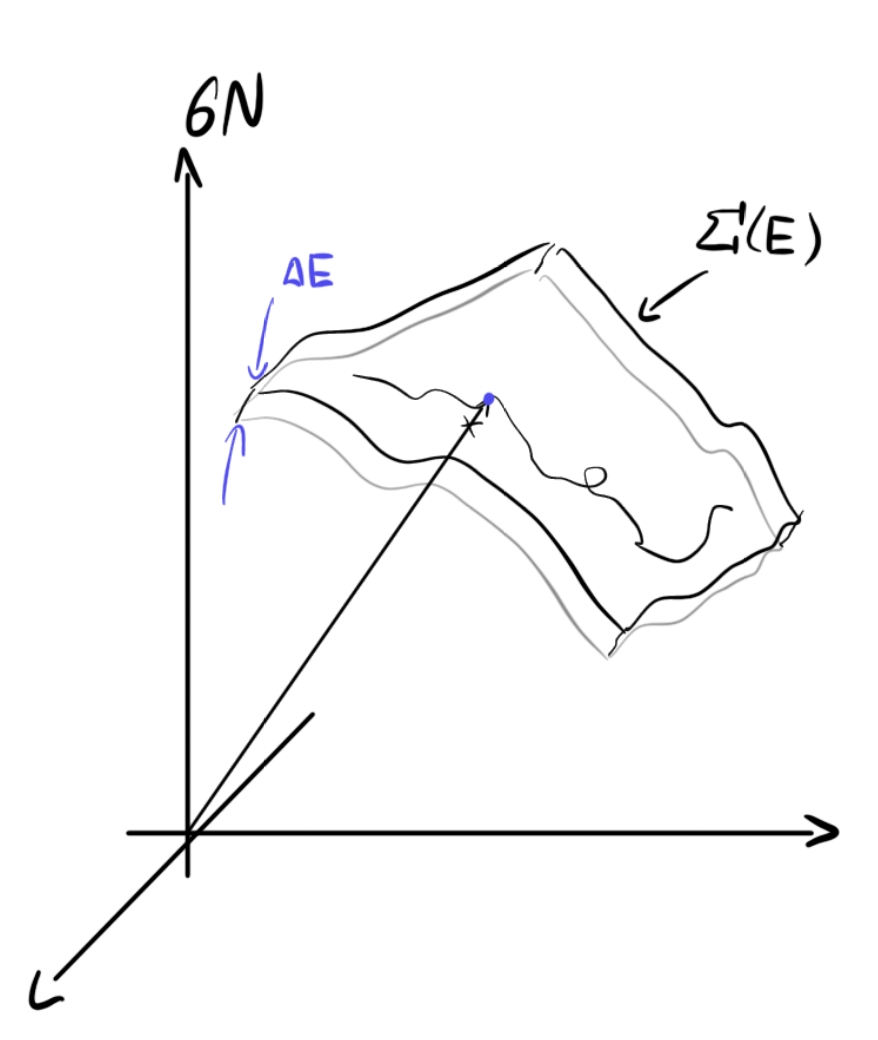
\includegraphics[width=0.4\textwidth]{images/1.jpg}
\end{center}

\subsection{Уравнения движения Гамильтона}

Движение изображающей точки в фазовом пространстве не является произвольным. Оно полностью детерминировано и подчиняется законам классической механики. В гамильтоновой формулировке эволюция системы описывается уравнениями Гамильтона:
\begin{equation}
    \dot{q}_i = \frac{\partial H}{\partial p_i}, \quad \dot{p}_i = -\frac{\partial H}{\partial q_i}
\end{equation}
Здесь $H(p, q)$ — гамильтониан системы, который в общем случае зависит от всех импульсов и координат частиц:
\begin{equation}
    H(p, q) = H(\vec{p}_1, \dots, \vec{p}_N, \vec{q}_1, \dots, \vec{q}_N)
\end{equation}
Гамильтониан представляет собой полную энергию системы, выраженную через переменные фазового пространства.

% Section 3: Геометрия фазового пространства изолированной системы
\section{Геометрия фазового пространства изолированной системы}

Теперь мы перейдем к рассмотрению важного частного случая — изолированной системы. В рамках микроканонического распределения мы будем формулировать законы именно для таких систем.

\subsection{Закон сохранения энергии и энергетическая гиперповерхность}

Основным свойством изолированной системы является закон сохранения энергии. Это означает, что гамильтониан системы в процессе движения остается постоянным и равным некоторому значению $E$:
\begin{equation}
    H(p, q) = E = \text{const}
\end{equation}
С геометрической точки зрения это уравнение накладывает связь на переменные $p$ и $q$, выделяя в $6N$-мерном фазовом пространстве многообразие меньшей размерности. Данное многообразие представляет собой гиперповерхность постоянной энергии, которую мы будем обозначать $\Sigma(E)$.

\subsection{Понятие энергетического слоя}

Лектор отмечает важный практический нюанс: точно задать энергию макроскопической системы $E$ с математической точностью практически невозможно. Такое представление является идеализацией. В реальности мы всегда знаем энергию системы лишь с некоторой конечной точностью $\Delta E$.

Поэтому правильнее говорить, что изображающая точка системы движется не строго по поверхности $\Sigma(E)$, а внутри некоторого тонкого слоя в фазовом пространстве. Этот слой, называемый энергетическим слоем или энергетической оболочкой, ограничен двумя гиперповерхностями, отвечающими энергиям $E$ и $E + \Delta E$.

Математически условие нахождения системы в таком слое записывается в виде неравенства:
\begin{equation}
    E \le H(p, q) \le E + \Delta E
\end{equation}
Мы предполагаем, что толщина этого слоя $\Delta E$ (неопределенность энергии) очень мала по сравнению с самой энергией системы:
\begin{equation}
    \Delta E \ll E
\end{equation}
Тем не менее, введение этого слоя принципиально важно для последующего статистического описания, так как оно позволяет говорить об объеме фазового пространства, доступном системе.


Изображающая точка движется в этом слое по крайне замысловатой траектории, многократно «наматываясь» и проходя через различные участки доступного фазового объема. Отследить это движение детально невозможно, да и не нужно, так как именно здесь на помощь приходят статистические методы.

% Section 4: Макросостояние и статистическое усреднение
\section{Макросостояние и статистическое усреднение}

Мы ввели понятие микроскопического состояния, которое задается точкой $P$ в фазовом пространстве, определяемой всеми импульсами и координатами системы:
\begin{equation}
    P = (p, q)
\end{equation}
Эта точка, как мы выяснили, движется по крайне сложной траектории в многомерном пространстве. Теперь необходимо соотнести это с тем, что мы наблюдаем в реальности.

\subsection{Определение макроскопического состояния через параметры (E, V, N)}

В отличие от микросостояния, макроскопическое состояние системы характеризуется небольшим набором параметров. Для изолированной системы в состоянии термодинамического равновесия такими параметрами являются:
\begin{itemize}
    \item Энергия системы $E$ (которую, как мы помним, мы знаем с точностью до энергетического слоя $\Delta E$);
    \item Объем системы $V$, в котором заключены частицы;
    \item Число частиц $N$.
\end{itemize}
Эти три величины $(E, V, N)$ полностью определяют макроскопическое состояние. Если система изолирована, эти параметры остаются постоянными, в то время как микросостояние $P(t)$ непрерывно и хаотично меняется.

\subsection{Проблема измерения физических величин}

Рассмотрим некоторую физическую величину $A$, которая является функцией микроскопического состояния системы:
\begin{equation}
    A = A(p, q)
\end{equation}
Примерами таких величин могут служить полная энергия, кинетическая энергия частиц, потенциальная энергия взаимодействия или давление. Поскольку изображающая точка системы перемещается в фазовом пространстве по некоторой траектории $p(t), q(t)$, то и сама физическая величина $A$ становится функцией времени:
\begin{equation}
    A(t) = A(p(t), q(t))
\end{equation}

\begin{center}
    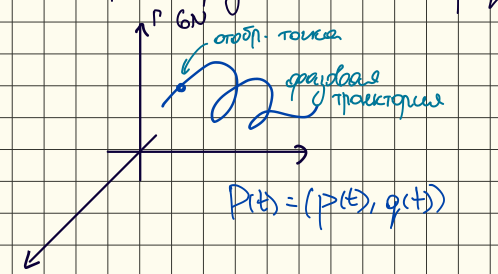
\includegraphics[width=0.5\textwidth]{images/3.png}
\end{center}

\subsection{Временное среднее значение величины}

Когда мы проводим физический эксперимент и измеряем величину $A$ прибором, мы не фиксируем её мгновенные микроскопические значения. Любой макроскопический прибор обладает инерционностью, и процесс измерения занимает конечное время $\tau$. То, что мы получаем на опыте — это среднее по времени значение величины:
\begin{equation}
    \bar{A} = \frac{1}{\tau} \int_0^\tau A(t) dt
\end{equation}
При этом время измерения $\tau$ в макроскопических масштабах огромно по сравнению с характерными микроскопическими временами (временем между столкновениями частиц или периодами колебаний атомов):
\begin{equation}
    \tau \gg t_{\text{микро}}
\end{equation}
Формально в теоретических выкладках мы можем считать, что время измерения стремится к бесконечности ($\tau \to \infty$). 

\subsection{Сложность отслеживания микроскопической динамики}

Главная проблема состоит в том, что для вычисления этого временного среднего значения нам необходимо знать точную фазовую траекторию системы, то есть решить уравнения Гамильтона для $10^{23}$ частиц. Это задача грандиозной сложности, и точное её решение не только невозможно, но и не нужно. Именно здесь возникает идея Гиббса о переходе от усреднения по времени к усреднению по некоторой совокупности состояний.

% Section 5: Метод статистических ансамблей
\section{Метод статистических ансамблей}

Для решения проблемы усреднения Джозайя Уиллард Гиббс предложил метод статистических ансамблей. Это ключевое понятие во всем нашем курсе.

\subsection{Понятие статистического ансамбля}

Статистический ансамбль — это огромное множество мысленных копий нашей системы. Все эти копии находятся в одном и том же макроскопическом состоянии (у них одинаковые $E, V, N$), но при этом они находятся в совершенно различных микроскопических состояниях. 

Представьте, что вместо того, чтобы следить за одной изображающей точкой, которая долго «бегает» по фазовому пространству, мы рассматриваем сразу всё множество возможных положений этой точки в данный момент времени. 

\begin{center}
    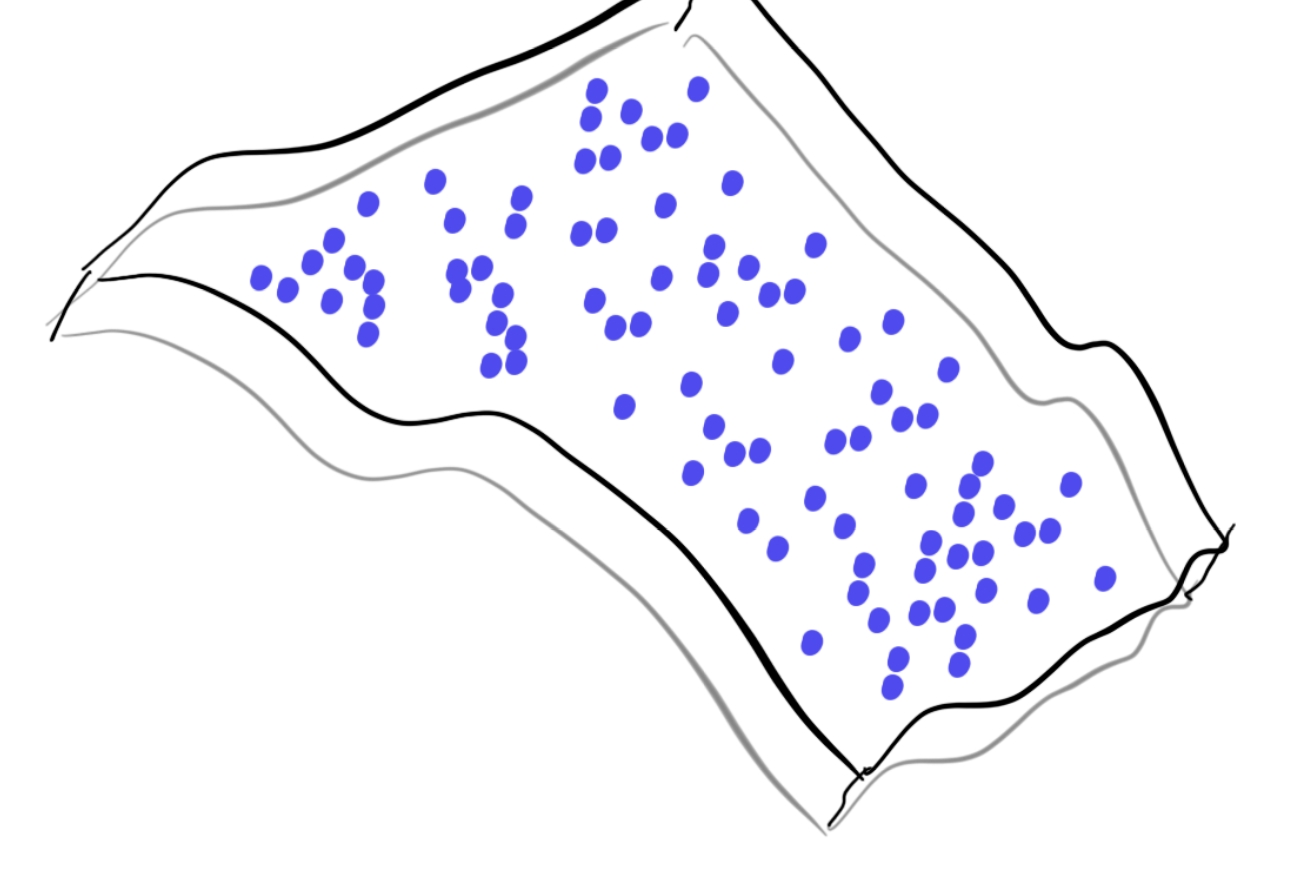
\includegraphics[width=0.5\textwidth]{images/4.jpg}
\end{center}

\subsection{Плотность распределения в фазовом пространстве}

Состояние ансамбля описывается плотностью распределения изображающих точек в фазовом пространстве $\rho(p, q)$. Эта величина определяет вероятность того, что система из ансамбля будет обнаружена в окрестности точки $(p, q)$ фазового пространства. Плотность распределения пропорциональна числу точек ансамбля в малом фазовом объеме:
\begin{equation}
    \rho(p, q) \sim \text{Вероятность обнаружить систему в состоянии } (p, q)
\end{equation}

Для равновесных систем плотность распределения не должна явно зависеть от времени:
\begin{equation}
    \frac{\partial \rho}{\partial t} = 0
\end{equation}
Это означает, что «облако» точек в фазовом пространстве может как-то перемещаться или деформироваться по законам механики, но его статистические характеристики в равновесии остаются неизменными.

\subsection{Эргодическая гипотеза}

Теперь мы можем сформулировать основной постулат, который связывает теорию с экспериментом. Это эргодическая гипотеза. Она утверждает, что среднее по времени значение величины $\bar{A}$, измеренное на опыте, совпадает со средним значением по статистическому ансамблю $\langle A \rangle$:
\begin{equation}
    \bar{A} = \langle A \rangle
\end{equation}
Усреднение по ансамблю (статистическое среднее) вычисляется по формуле:
\begin{equation}
    \langle A \rangle = \frac{\int A(p, q) \rho(p, q) d\Gamma}{\int \rho(p, q) d\Gamma}
\end{equation}
Здесь интеграл берется по всему фазовому пространству $d\Gamma$. Это утверждение является фундаментом статистической физики. Оно позволяет заменить невыполнимое прослеживание траектории одной системы во времени вычислением интегралов по состояниям множества систем.

\subsection{Нормировка плотности распределения}

Для удобства мы будем использовать нормированную плотность распределения. Если мы обозначим ненормированную функцию как $\rho_0(p, q)$, то нормированная функция $\rho$ определяется так, чтобы её интеграл по всему доступному фазовому пространству был равен единице:
\begin{equation}
    \int \rho(p, q) d\Gamma = 1
\end{equation}
Тогда формула для среднего упрощается:
\begin{equation}
    \langle A \rangle = \int A(p, q) \rho(p, q) d\Gamma
\end{equation}
Остается главный вопрос: как найти вид этой функции $\rho(p, q)$ для конкретных физических условий? Этим мы займемся далее.

% Section 6: Микроканоническое распределение
\section{Микроканоническое распределение}

Теперь мы переходим к центральному вопросу: как же нам найти плотность распределения $\rho(p, q)$ для изолированной системы? На самом деле, точного аналитического вывода этой функции из уравнений механики не существует, поэтому в основу статистической физики кладется фундаментальное предположение.

\subsection{Постулат о равновероятности микросостояний}

Этот постулат является «краеугольным камнем» метода ансамблей Гиббса для изолированных систем. Он формулируется следующим образом:

\begin{quote}
    Для изолированной системы, находящейся в состоянии термодинамического равновесия, все \textit{допустимые} микросостояния равновероятны.
\end{quote}

Что здесь означает слово «допустимые»? Это те состояния, которые совместимы с наложенными на систему макроскопическими условиями. Для изолированной системы это означает, что энергия системы должна лежать в заданном интервале (энергетическом слое). То есть допустимыми являются те точки фазового пространства, для которых:
\begin{equation}
    E \le H(p, q) \le E + \Delta E
\end{equation}

\subsection{Математическая запись плотности распределения}

Из этого постулата сразу следует вид плотности распределения. Сначала введем ненормированную функцию распределения, которую обозначим $\rho^*(p, q)$. Раз все допустимые состояния равновероятны, то внутри слоя плотность должна быть константой (для простоты примем её за единицу), а вне слоя — нулю, так как система там находиться не может:

\begin{equation}
    \rho^*(p, q) = 
    \begin{cases} 
      1, & E \le H(p, q) \le E + \Delta E \\
      0, & \text{вне этого слоя}
    \end{cases}
\end{equation}


\subsection{Нормировка и статистический вес $\Omega(E)$}

Чтобы получить физически осмысленную плотность распределения $\rho$, её нужно нормировать на единицу. Для этого мы должны разделить $\rho^*$ на полный фазовый объем, занимаемый ансамблем. Этот объем (интеграл от плотности по всему фазовому пространству) мы обозначим $\Delta \Gamma$:

\begin{equation}
    \Delta \Gamma = \int \rho^*(p, q) d\Gamma = \int_{E \le H \le E + \Delta E} d\Gamma
\end{equation}

Эту величину в статистической физике называют \textbf{статистическим весом} данного макросостояния и часто обозначают символом $\Omega(E)$. Таким образом, окончательная формула для \textbf{микроканонического распределения} принимает вид:

\begin{equation}
    \rho^{\text{МКР}}(p, q) = 
    \begin{cases} 
      \frac{1}{\Omega(E)}, & E \le H(p, q) \le E + \Delta E \\
      0, & \text{вне этого слоя}
    \end{cases}
\end{equation}

Эта функция дает нам вероятность найти систему в единичном фазовом объеме около точки $(p, q)$. 

% Section 7: Основные статистические функции
\section{Основные статистические функции}

Для работы с микроканоническим распределением нам необходимо ввести несколько крайне важных функций, которыми мы будем постоянно пользоваться.

\subsection{Фазовый интеграл $\Gamma(E)$}

Введем функцию $\Gamma(E)$, которую будем называть \textbf{фазовым интегралом}. Она определяется как полный объем фазового пространства, ограниченный гиперповерхностью с энергией $E$:
\begin{equation}
    \Gamma(E) = \int_{H(p, q) \le E} d\Gamma
\end{equation}
То есть это «суммарный объем», в котором энергия системы не превышает значения $E$.

\textit{Важное замечание лектора:} Пожалуйста, не путайте обозначение функции $\Gamma(E)$ с обозначением самого фазового пространства (Г-пространства). К сожалению, в литературе часто используется одна и та же греческая буква, но смысл у них разный: одно — это само пространство, а другое — функция энергии (объем).

\subsection{Плотность состояний $D(E)$}

Следующая фундаментальная величина — плотность состояний $D(E)$. По определению, это производная от фазового интеграла по энергии:
\begin{equation}
    D(E) = \frac{d\Gamma(E)}{dE}
\end{equation}
Физически $D(E)$ показывает, как много микросостояний приходится на единичный интервал энергии. Используя это определение, мы можем связать статистический вес $\Omega(E)$ с плотностью состояний. Так как $\Omega(E)$ — это объем тонкого слоя толщиной $\Delta E$, то:
\begin{equation}
    \Omega(E) = \Gamma(E + \Delta E) - \Gamma(E) \approx D(E) \Delta E
\end{equation}

\subsection{Безразмерный элемент фазового объема и тождественность частиц}

До сих пор мы писали $d\Gamma$ как произведение дифференциалов координат и импульсов. Однако, чтобы результаты были корректными и в дальнейшем согласовывались с квантовой механикой (например, для идеального газа), нам нужно сделать фазовый объем безразмерным и учесть тождественность частиц.

Правильное определение безразмерного элемента фазового объема выглядит так:
\begin{equation}
    d\Gamma = \frac{1}{N!} \frac{\prod_{i=1}^N d^3 p_i d^3 q_i}{(2\pi\hbar)^{3N}}
\end{equation}
Здесь мы добавили:
\begin{enumerate}
    \item Множитель $1/N!$ — он учитывает, что перестановка двух одинаковых (тождественных) частиц не меняет физического состояния системы. Без этого множителя мы получили бы парадокс Гиббса (неаддитивность энтропии).
    \item Постоянную Планка в степени $3N$ — это делает величину безразмерной. Каждому квантовому состоянию в классическом пределе соответствует ячейка фазового объема размером $(2\pi\hbar)^3$ на одну частицу.
\end{enumerate}

В дальнейшем под символом $\int \dots d\Gamma$ мы всегда будем подразумевать интегрирование с учетом этих множителей.

% Section 8: Статистическая энтропия
\section{Статистическая энтропия}

Мы ввели основные понятия: микроканоническое распределение, статистический вес и плотность состояний. Теперь мы готовы сделать шаг к термодинамике и ввести фундаментальную величину — энтропию.

\subsection{Энтропия и формула Больцмана}

В статистической физике энтропия определяется через микроскопические характеристики системы. Фундаментальное соотношение, которое вводит энтропию, называется формулой Больцмана. Согласно этой формуле, энтропия $S$ есть логарифм статистического веса $\Omega(E)$:

\begin{equation}
    S = \ln \Omega(E)
\end{equation}

Иногда удобно использовать для определения энтропии фазовый интеграл $\Gamma(E)$, то есть логарифм объема фазового пространства, ограниченного энергией $E$:

\begin{equation}
    S = \ln \Gamma(E)
\end{equation}

На физическом уровне строгости можно показать, что при макроскопически большом числе частиц ($N \to \infty$) эти два определения эквивалентны, так как основная часть фазового объема сосредоточена вблизи его границы. Мы будем считать это эквивалентными формами записи. Эта формула является основой основ нашей науки.

\subsection{Свойство аддитивности энтропии}

Важнейшим свойством энтропии является её аддитивность. Энтропия является функцией экстенсивных переменных: энергии системы $E$, объема $V$ и числа частиц $N$:

\begin{equation}
    S = S(E, V, N)
\end{equation}

Поскольку энтропия пропорциональна числу частиц в системе (при фиксированных удельных величинах), мы можем записать её в виде:

\begin{equation}
    S = N \cdot s\left(\frac{V}{N}, \frac{E}{N}\right)
\end{equation}

Здесь $s$ — удельная энтропия, которая зависит только от удельного объема и удельной энергии. Это свойство — аддитивность — крайне важно. Представьте, что мы привели две одинаковые системы в тепловой контакт, они находятся в равновесии. Если мы удвоим все параметры ($E, V, N$), то энтропия системы тоже удвоится.

Мы не будем здесь глубоко погружаться в доказательство этого факта на основе эргодической гипотезы — это заняло бы слишком много времени. Мы принимаем формулу Больцмана как данность и будем из неё выводить все остальные равновесные свойства.

% Section 9: Применение метода: Идеальный газ Больцмана
\section{Применение метода: Идеальный газ Больцмана}

Чтобы оправдать введение всех этих сложных понятий, давайте рассмотрим пример, где всё вычисляется до конца. Это пример классического идеального газа Больцмана.

\subsection{Гамильтониан идеального газа}

Для идеального газа мы предполагаем, что потенциальная энергия взаимодействия между частицами пренебрежимо мала. Гамильтониан такой системы представляет собой просто сумму кинетических энергий всех атомов:

\begin{equation}
    H(p, q) = \sum_{i=1}^N \frac{\vec{p}_i^2}{2m}
\end{equation}

Заметим важную особенность: гамильтониан здесь не зависит от координат частиц $\vec{q}_i$. Это значительно упрощает расчеты.

\subsection{Вычисление фазового интеграла}

Нам нужно вычислить фазовый интеграл $\Gamma(E)$. Вспомним определение безразмерного элемента объема:

\begin{equation}
    \Gamma(E) = \int_{H \le E} \frac{1}{N!} \frac{\prod d^3 p_i d^3 q_i}{(2\pi\hbar)^{3N}}
\end{equation}

Поскольку интегрирование по координатам и импульсам разделяется, мы можем сначала проинтегрировать по всем $d^3 q_i$. Каждая частица может находиться в любой точке объема $V$, поэтому каждый интеграл $\int d^3 q_i$ дает нам $V$. Всего у нас $N$ таких интегралов, что дает множитель $V^N$:

\begin{equation}
    \Gamma(E) = \frac{V^N}{N! (2\pi\hbar)^{3N}} \int_{\sum p_i^2 \le 2mE} d^{3N} p
\end{equation}

Оставшийся интеграл по импульсам имеет ясный геометрический смысл. Условие $\sum_{i=1}^N (p_{ix}^2 + p_{iy}^2 + p_{iz}^2) \le 2mE$ — это уравнение шара в пространстве импульсов. Поскольку у нас $N$ частиц и у каждой 3 компоненты импульса, это шар в пространстве размерности $n = 3N$. Радиус этого шара равен $R = \sqrt{2mE}$.

\subsection{Объем многомерного шара}

Объем $n$-мерного шара радиуса $R$ пропорционален $R^n$:
\begin{equation}
    V_n(R) = C_n R^n
\end{equation}
Коэффициент пропорциональности $C_n$ зависит от размерности пространства. Лектор приводит результат для этого коэффициента (это стандартный результат, который можно найти в справочниках или вывести через Гамма-функции):

\begin{equation}
    C_n = \frac{\pi^{n/2}}{\Gamma(\frac{n}{2} + 1)}
\end{equation}

В нашем случае $n = 3N$. При очень больших $N$ мы можем воспользоваться формулой Стирлинга для Гамма-функции: $\ln \Gamma(x+1) \approx x \ln(x/e)$. После подстановки всех величин и упрощения выражения для объема $3N$-мерного шара импульсов, мы получаем:

\begin{equation}
    V_{3N} \approx \left( \frac{4\pi m e E}{3N} \right)^{3N/2}
\end{equation}


\subsection{Итоговое выражение для энтропии}

Собирая все множители вместе и применяя формулу Стирлинга $\ln N! \approx N\ln(N/e)$ к факториалу, мы получаем итоговое выражение для энтропии идеального газа:

\begin{equation}
    S(E, V, N) = N \ln \left[ \frac{eV}{N(2\pi\hbar)^3} \left( \frac{4\pi m e E}{3N} \right)^{3/2} \right]
\end{equation}

Это и есть формула Больцмана–Гиббса для энтропии классического идеального газа (в несколько иной форме известная как формула Саккура–Тетроде). Энтропия аддитивна: она пропорциональна $N$, а под логарифмом стоят удельные величины $V/N$ и $E/N$. На следующей лекции мы установим связь этого выражения с термодинамикой и выведем из него температуру, давление и химический потенциал. Спасибо за внимание.

\end{document}
